\documentclass[11pt,class=report,crop=false]{standalone}
\usepackage[screen]{../python}


\begin{document}


%====================================================================
\chapitre{Logarithme}
%====================================================================

\index{logarithme}

\objectifs{Le logarithme est une fonction aussi importante que l'exponentielle. C'est le logarithme qui donne l'ordre de grandeur de certaines quantités physiques, par exemple la puissance d'un séisme ou celle d'un son.}


\myfigure{0.8}{
\tikzinput{fig_logarithme_01}
}

\bigskip



%%%%%%%%%%%%%%%%%%%%%%%%%%%%%%%%%%%%%%%%%%%%%%%%%%%%%%%%%%%%%%%%
%%%%%%%%%%%%%%%%%%%%%%%%%%%%%%%%%%%%%%%%%%%%%%%%%%%%%%%%%%%%%%%%

\begin{cours}[Le logarithme décimal]

\index{logarithme!decimal@décimal}

On commence avec le logarithme décimal qui est plus facile à appréhender.
Le logarithme décimal d'un nombre réel positif $x$, est l'exposant $y$ de ce nombre écrit sous la forme $x=10^y$.
Autrement dit :
\mybox{$x = 10^y \quad \iff \quad y = \log_{10}(x)$}

\textbf{Exemples.}

\begin{itemize}
  \item $\log_{10}(10^2) = 2$, $\log_{10}(10^3) = 3$, $\log_{10}(10\,000) = 4$,\ldots
  \item On a aussi $\log_{10}(10)=1$, $\log_{10}(1)=0$.
  \item Comme $0.1 = \frac{1}{10} = 10^{-1}$, on a $\log_{10}(0.1)=-1$.
  \item Le logarithme est défini pour n'importe quel $x>0$.
  Par exemple pour $x = 25.5$, on a $\log_{10}(x) = 1.4065\ldots$
  Ce qui signifie que $10^{1.4065\ldots} = 25.5$.

  \end{itemize}

\textbf{Propriété.}
La propriété fondamentale du logarithme est :
\mybox{$\log_{10}(a \times b) = \log_{10}(a) + \log_{10}(b)$}

Par exemple $a = 10^2$, $b=10^3$, on a $a\times b  = 10^2 \times 10^3 = 10^{2+3} = 10^5$. On a bien 
$$\log_{10}(a) + \log_{10}(b) = \log_{10}(10^2) + \log_{10}(10^3)
= 2+3 = 5 = \log_{10}(10^5)= \log_{10}(a \times b) $$


\end{cours}

%%%%%%%%%%%%%%%%%%%%%%%%%%%%%%%%%%%%%%%%%%%%%%%%%%%%%%%%%%%%%%%%
%%%%%%%%%%%%%%%%%%%%%%%%%%%%%%%%%%%%%%%%%%%%%%%%%%%%%%%%%%%%%%%%


\begin{cours}[Le(s) logarithme(s) avec \Python]
\sauteligne

\objectifs{Avertissement : il y a un conflit entre mathématiciens et informaticiens pour la notation du logarithme !}

\index{log@\ci{log}}

\begin{itemize}
  \item \textbf{Logarithme décimal.}
  \begin{itemize} 
    \item Notation mathématique : $\log_{10}(x)$
    \item Commande \Python{} : \ci{log(x,10)}
  \end{itemize}
  
   \item \textbf{Logarithme népérien.}
  \begin{itemize} 
    \item Notation mathématique : $\ln(x)$
    \item Commande \Python{} : \ci{log(x)}
  \end{itemize}
  
    \item \textbf{Logarithme en une autre base.}
  \begin{itemize} 
    \item Notation mathématique : $\log_b(x)$
    \item Commande \Python{} : \ci{log(x,b)}
  \end{itemize} 
   
\end{itemize}

Exemple : avec $x = 25.5$, alors on calcule $\log_{10}(x)$ par la commande
\ci{log(25.5,10)} qui renvoie 
$$\log_{10}(x) \simeq 1.406540180433955$$
On vérifie le résultat en calculant $10^y$, où $y=1.4065\ldots$ par la commande \ci{10**y} qui renvoie :
$$25.49999999999999$$
Bien sûr, tous les calculs effectués par \Python{} avec les nombres flottants
sont des calculs approchés.
\end{cours}


%%%%%%%%%%%%%%%%%%%%%%%%%%%%%%%%%%%%%%%%%%%%%%%%%%%%%%%%%%%%%%%%
% Activité 1 - Logarithme décimal - Échelle de Richter
%%%%%%%%%%%%%%%%%%%%%%%%%%%%%%%%%%%%%%%%%%%%%%%%%%%%%%%%%%%%%%%%

\begin{activite}[Logarithme décimal - Échelle de Richter]
   
\objectifs{Objectifs : comprendre l'échelle de Richter qui mesure la force d'un tremblement de terre.}

On quantifie la force d'un séisme par un nombre, appelé \defi{magnitude}, qui dépend de la puissance délivrée par une secousse :
$$M = \frac{2}{3} \log_{10} \left(\frac{E}{E_0} \right) - 3.2$$
où :
\begin{itemize}
  \item $\log_{10}$ est le logarithme décimal,
  \item $E$ est l'énergie délivrée par le séisme (exprimée en joules),
  \item $E_0 = 1.6 \times 10^{-5}$ joules est une énergie de référence.
\end{itemize}  
  
 {\small
\begin{center}
\begin{tabular}{|l|c|p{8cm}|c|}
\hline
Description &	Magnitude &	Effets &Fréquence moyenne \\ \hline\hline
Micro &	moins de 1.9 &	Micro tremblement de terre, non ressenti. &	8 000 par jour\\ \hline
Très mineur &	2.0 à 2.9 &	Généralement non ressenti mais détecté/enregistré. &	1 000 par jour\\ \hline
Mineur& 	3.0 à 3.9& 	Souvent ressenti sans causer de dommages. &	50 000 par an\\ \hline
Léger &	4.0 à 4.9 &	Secousses notables d'objets à l'intérieur des maisons, bruits d'entrechoquement. Les dommages restent très légers. &	6 000 par an\\ \hline
Modéré &	5.0 à 5.9 &	Peut causer des dommages significatifs à des édifices mal conçus dans des zones restreintes. Pas de dommages aux édifices bien construits. &	800 par an\\ \hline
Fort &	6.0 à 6.9 &	Peut provoquer des dommages sérieux sur plusieurs dizaines de kilomètres. Seuls les édifices adaptés résistent près du centre. &	120 par an\\ \hline
Très fort &	7.0 à 7.9 &	Peut provoquer des dommages sévères dans de vastes zones ; tous les édifices sont touchés près du centre. &	18 par an\\ \hline
Majeur &	8.0 à 8.9 &	Peut causer des dommages très sévères dans des zones à des centaines de kilomètres à la ronde. Dommages majeurs sur tous les édifices, y compris à des dizaines de kilomètres du centre. &	1 par an\\ \hline
Dévastateur & 9.0 et plus &	Dévaste des zones sur des centaines de kilomètres à la ronde. Dommages sur plus de 1 000 kilomètres à la ronde. &	1 à 5 par siècle \\ \hline
\end{tabular}

\smallskip

\emph{Source : \og{}Magnitude (Sismologie)\fg{}  Wikipédia.}
\end{center}  
}
  \begin{enumerate}
    \item Programme une fonction \ci{magnitude(E)} qui renvoie la magnitude d'un séisme dont l'énergie $E$ est donnée.
    
    \emph{Exemple.} Vérifie qu'un séisme libérant une énergie $E_1 = 10^6$ joules est de magnitude $4$.
    
    \item Pour des énergies de la forme $E = 10^i$, calcule la magnitude correspondante jusqu'à obtenir un séisme de magnitude supérieure à $9$.
    
    \item Par tâtonnement, balayage ou en résolvant une équation, trouve l'énergie environ nécessaire pour obtenir un séisme de magnitude $7$.
    
    \item Vérifie expérimentalement, puis montre mathématiquement, que si $E_2 = 1000 E_1$ alors 
    $M_2 = M_1 + 2$ (quelle que soit l'énergie $E_1$).
    Trouve expérimentalement (ou mathématiquement) quel facteur $k$, avec $E_2 = k E_1$ 
    permet d'obtenir $M_2 = M_1 + 1$ (quelle que soit l'énergie $E_1$).
    
  \end{enumerate}
 
\end{activite}

%%%%%%%%%%%%%%%%%%%%%%%%%%%%%%%%%%%%%%%%%%%%%%%%%%%%%%%%%%%%%%%%
% Activité 2 - Logarithme décimal - Décibels
%%%%%%%%%%%%%%%%%%%%%%%%%%%%%%%%%%%%%%%%%%%%%%%%%%%%%%%%%%%%%%%%


\begin{activite}[Logarithme décimal - Décibels]

\objectifs{Objectifs : calculer le niveau sonore.}

On mesure le niveau de bruit en décibels (dB) qui correspond à la puissance d'un son (par rapport à une puissance de référence). La formule est 
$$D = 20 \log_{10} \left(\frac{P}{P_0} \right)$$
où :
\begin{itemize}
  \item $\log_{10}$ est le logarithme décimal,
  \item $P$ est la pression mesurée du son (exprimée en pascal Pa),
  \item $P_0 = 2 \times 10^{-5}$ Pa est une pression de référence.
\end{itemize}  


  \begin{enumerate}
    \item Programme une fonction \ci{decibels(P)} qui renvoie le niveau de bruit d'un son de puissance $P$ donnée.
    
    \emph{Exemple.} Vérifie qu'une puissance $P = 1$ Pa, correspond à $D = 94$ décibels.    
    
    \item Complète le tableau suivant :
    

\begin{center}
\begin{tabular}{|c|c|c|}
\hline
Bruit &	Pression (Pa) &	Niveau (dB)  \\ \hline\hline

Moteur d'avion à réaction (à 1 mètre) & 632 & \\\hline
Marteau-piqueur (à 1 mètre) & 2 & \\\hline
Niveau de dommage à l'oreille & P > 0.355 & \\\hline
Niveau de gêne & & D > 70 \\\hline
Conversation (à 1 mètre) &  0.002 à 0.02 & \\\hline
Chambre calme & &  10 à 20 \\\hline
Seuil de l'audition à 1kHz (à l'oreille) &  $2 \cdot 10^{-5}$ & \\\hline
Chambre anéchoïque & &  $-10$ \\ \hline
\end{tabular}

\smallskip 

\emph{Source : \og{}Sound pressure\fg{}  Wikipédia.}
\end{center}  
   
  \end{enumerate}
 
\end{activite}

%%%%%%%%%%%%%%%%%%%%%%%%%%%%%%%%%%%%%%%%%%%%%%%%%%%%%%%%%%%%%%%%
%%%%%%%%%%%%%%%%%%%%%%%%%%%%%%%%%%%%%%%%%%%%%%%%%%%%%%%%%%%%%%%%

\begin{cours}[Échelle logarithmique]

\textbf{Relation $y=ax+b$.}
On considère des données du type $(x_i,y_i)$ et on veut étudier le lien entre $y_i$ et $x_i$.
On détecte facilement une relation affine du type $y=ax+b$ en plaçant les points sur un graphique. Une telle relation existe si et seulement si les points sont tous sur une même droite.


Ci-dessous des points vérifiant la relation $y = \frac12 x +1$.
\myfigure{0.8}{
\tikzinput{fig_echelle_01}
}

\textbf{Relation $y=10^{ax+b}$.}
Les données sont du type $(x_i,y_i)$ mais cette fois la relation est du type  $y=10^{ax+b}$.
Si on trace les points directement sous la forme $(x,y)$ on ne voit rien de spécial (figure ci-dessous à gauche\couleurnb{, les points rouges}{}). Par contre si on place les points $(x,\log_{10}(y))$ alors les points sont alignés (figure ci-dessous à droite\couleurnb{, les points verts}{}). (Preuve : comme $y=10^{ax+b}$ alors $\log_{10}(y) = ax+b$.)

Ci-dessous des points vérifiant la relation $y = 10^{\tfrac15 x -1}$.
\myfigure{0.65}{
\tikzinput{fig_echelle_02}\qquad
\tikzinput{fig_echelle_03}
}


\textbf{Relation $y=b x^a$.}
Les données sont du type $(x_i,y_i)$ avec la relation $y=bx^a$.
Le tracé des points $(x,y)$ ne donne rien (figure ci-dessous à gauche\couleurnb{, les points rouges}{}). 
Par contre le tracé des points $(\log_{10}(x),\log_{10}(y))$ donne des points alignés (figure ci-dessous à droite\couleurnb{, les points bleus}{}). (Preuve : comme $y=bx^a$ alors $\log_{10}(y) = \log_{10}(bx^a)$ donc
$\log_{10}(y) = \log_{10}(b) + \log_{10}(x^a)$, d'où $\log_{10}(y) = a\log_{10}(x)+\log_{10}(b)$. Si on pose $Y=\log_{10}(y)$ et $X=\log_{10}(x)$ on trouve une relation affine $Y=aX+ \log_{10}(b)$.)


Ci-dessous des points vérifiant la relation $y = 2x^{\frac12}$ (c'est-à-dire $y=2\sqrt{x}$).
\myfigure{0.6}{
\tikzinput{fig_echelle_04}\qquad
\tikzinput{fig_echelle_05}
}


\end{cours}


%%%%%%%%%%%%%%%%%%%%%%%%%%%%%%%%%%%%%%%%%%%%%%%%%%%%%%%%%%%%%%%%
% Activité 3 - Le logarithme décimal - Échelle logarithmique
%%%%%%%%%%%%%%%%%%%%%%%%%%%%%%%%%%%%%%%%%%%%%%%%%%%%%%%%%%%%%%%%


\begin{activite}[Le logarithme décimal - Échelle logarithmique]

\objectifs{Objectifs : utiliser le logarithme pour détecter des comportements particuliers.}


  \begin{enumerate}
    \item 
    \begin{itemize}
      \item Programme une fonction \ci{afficher_points_xy(points)} qui affiche (en rouge) chaque point de coordonnées $(x,y)$ à partir d'une liste de points.
      \item Programme une fonction \ci{afficher_points_xlogy(points)} qui affiche (en vert) chaque point de coordonnées $(x,\log_{10}(y))$ à partir d'une liste de points $(x,y)$ donnée.
      \item Programme une fonction \ci{afficher_points_logxlogy(points)} qui affiche (en bleu) chaque point de coordonnées $(\log_{10}(x),\log_{10}(y))$ à partir d'une liste de points $(x,y)$ donnée.
    \end{itemize}
    
        
    \item  Voici trois séries de données $(x,y)$ :
    
    $$
     \begin{array}{|c|c|}
    \hline
    x & y \\ \hline\hline
    2 & 5.66 \\ \hline
    3 & 10.39 \\ \hline
    5 & 22.36 \\ \hline
    7 & 37.04 \\ \hline
    11 & 72.97 \\ \hline                
    \end{array}\qquad \qquad  
    \begin{array}{|c|c|}
    \hline
    x & y \\ \hline\hline
    2 & 5 \\ \hline
    3 & 6.5 \\ \hline
    5 & 9.5 \\ \hline
    7 & 12.5 \\ \hline
    11 & 18.5 \\ \hline                
    \end{array}\qquad \qquad
    \begin{array}{|c|c|}
    \hline
    x & y \\ \hline\hline
    2 & 5.01 \\ \hline
    3 & 6.31 \\ \hline
    5 & 10.00 \\ \hline
    7 & 15.84 \\ \hline
    11 & 39.81 \\ \hline                
    \end{array}  
    $$    
    
    \medskip
    
    Reconnais par affichage graphique, celle qui est de la forme $y=ax+b$,
    celle qui est de la forme $y = 10^{ax+b}$ et celle de la forme $y = b x^a$.
    
    \emph{Bonus.} Calcule les constantes $a$ et $b$ qui conviennent dans chacun des cas.
   
    
  \end{enumerate}


\emph{Utiliser Matplolib.} Voici un bref programme qui affiche un point rouge de coordonnées $(2,5)$ et un point bleu de coordonnées $(7,2)$. 

\begin{minipage}{0.4\textwidth}
\begin{lstlisting}
import matplotlib.pyplot as plt
plt.scatter(2,5,color="red")
plt.scatter(7,2,color="blue")
plt.axes().set_aspect('equal')
plt.xlim(xmin=0)
plt.ylim(ymin=0)
plt.grid()
plt.show()
\end{lstlisting}
\end{minipage}\quad
\begin{minipage}{0.55\textwidth}
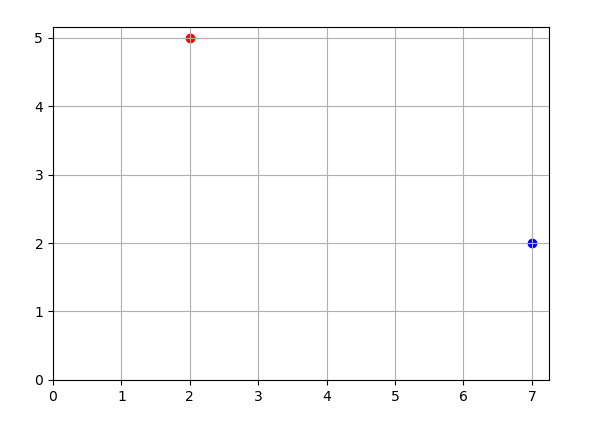
\includegraphics[scale=\myscale,scale=0.4]{ecran_logarithme_1}
\end{minipage}
\end{activite}



%%%%%%%%%%%%%%%%%%%%%%%%%%%%%%%%%%%%%%%%%%%%%%%%%%%%%%%%%%%%%%%%
%%%%%%%%%%%%%%%%%%%%%%%%%%%%%%%%%%%%%%%%%%%%%%%%%%%%%%%%%%%%%%%%


\begin{cours}[Logarithme népérien]
\sauteligne


\myfigure{0.8}{
	\tikzinput{fig_logarithme_01}
}

\index{logarithme!neperien@népérien}

\begin{itemize}
  \item La \defi{fonction logarithme népérien} est la fonction $\ln : ]0,+\infty[ \to \Rr$ qui vérifie :
  
  \smallskip
  
  \mybox{$\ln(1) = 0 \qquad \text{ et } \qquad \ln(x \times y) = \ln(x) + \ln(y)$}

  \item La fonction logarithme est strictement croissante,
  $\lim_{x\to 0^+} \ln(x) = -\infty$, \ $\lim_{x\to+\infty} \ln(x) = +\infty$.
    
  \item $\ln(1/x) = -\ln(x)$, \ $\ln(x^n) = n\ln(x)$.

  \item La dérivée du logarithme est : $\ln'(x) = \frac1x$.
  
  \item La fonction logarithme $\ln : ]0,+\infty[ \to \Rr$ est la bijection réciproque de la fonction exponentielle $\exp : \Rr \to ]0,+\infty[$, c'est-à-dire :
  \mybox{$y = \ln(x) \iff x = \exp(y)$}
  
  Plus précisément :
  $$\exp\big(\ln(x) \big) \qquad \text{ pour tout } x >0,$$
  $$\ln\big(\exp(x) \big) \qquad \text{ pour tout } x \in \Rr.$$
  
  
  \item On note $e=\exp(1) = 2.718\ldots$ et alors $\ln(e)=1$. 
    
  \item Le logarithme et l'exponentielle permettent de définir une puissance avec des exposants réels :
   $a^b = \exp\big(b \ln(a) \big)$.
  \end{itemize}
  
  
\end{cours}

%%%%%%%%%%%%%%%%%%%%%%%%%%%%%%%%%%%%%%%%%%%%%%%%%%%%%%%%%%%%%%%%
%%%%%%%%%%%%%%%%%%%%%%%%%%%%%%%%%%%%%%%%%%%%%%%%%%%%%%%%%%%%%%%%


\begin{cours}[Tables de logarithmes]
\sauteligne

Le logarithme a été introduit au début des années 1600 pour effectuer facilement des multiplications à plusieurs chiffres nécessaires aux calculs astronomiques.

\begin{center}
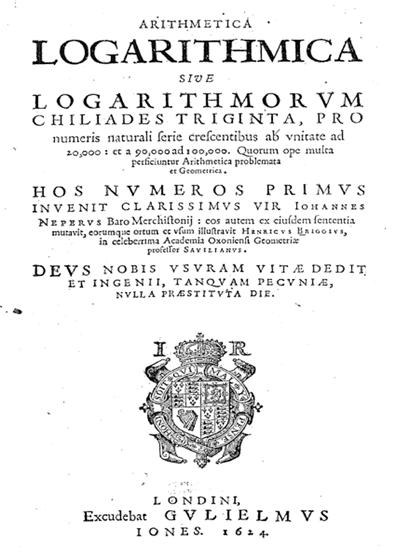
\includegraphics[scale=\myscale,scale=0.55,angle=-0.5]{briggs_1}\qquad\qquad
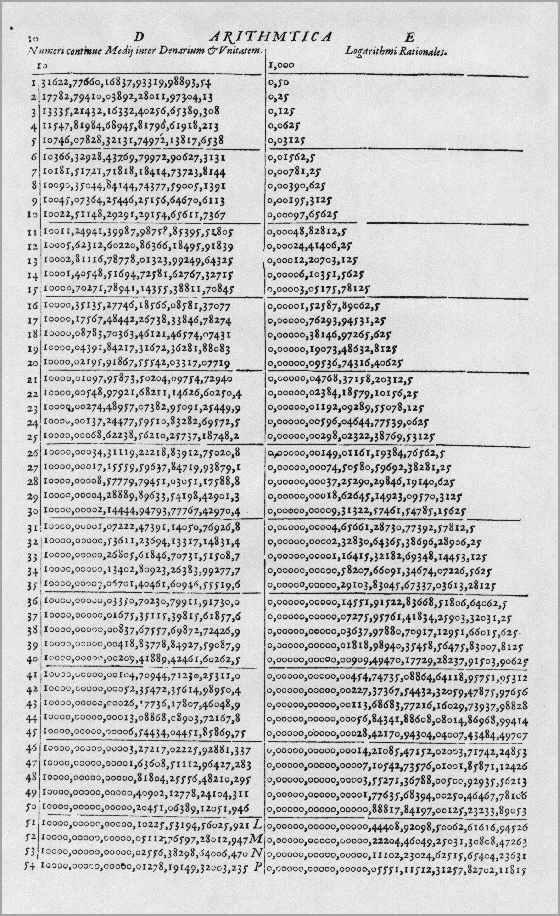
\includegraphics[scale=\myscale,scale=0.25]{briggs_2}

\emph{\og{}Arithmetica logarithmica\fg{} Tables de logarithmes de H.~Briggs, 1624.}
\end{center}


\textbf{Tables de logarithmes.}

Le préalable est de calculer une table des logarithmes, c'est-à-dire 
les valeurs approchées de $\ln(x)$ pour plein de valeurs de $x$.
Par exemple, voici le début d'une table de logarithme avec $4$ décimales après la virgule :
$$\begin{array}{|c|c|}
\hline
x & y=\ln(x) \\ \hline\hline
1.000 & 0.0000 \\ \hline
1.001 & 0.0010 \\ \hline
\cdots & \cdots \\ \hline
1.123 & 0.1160 \\ \hline
1.124 & 0.1169 \\ \hline
\cdots & \cdots \\ \hline
2.000 & 0.6931 \\ \hline
2.001 & 0.6936 \\ \hline 
2.002 & 0.6941 \\ \hline
\cdots & \cdots \\ \hline
\end{array}\qquad\qquad
\begin{array}{|c|c|}
\hline
x & y=\ln(x) \\ \hline\hline
\cdots & \cdots \\ \hline
2.567 & 0.9427 \\ \hline
2.568 & 0.9431 \\ \hline
\cdots & \cdots \\ \hline
2.718 & 0.9999 \\ \hline
2.719 & 1.0003 \\ \hline
\cdots & \cdots \\ \hline
2.884 & 1.0592  \\ \hline
2.885 & 1.0595  \\ \hline
2.886 & 1.0599  \\ \hline
\cdots & \cdots \\ \hline
\end{array}$$
 
 
\bigskip

\textbf{Lecture de la table.}

 \begin{itemize}
  \item Pour chercher le logarithme d'un nombre $x$ il suffit de consulter la table de la gauche vers la droite. Par exemple, on lit que pour $x=1.123$ on a $\ln(x) \simeq 0.1160$.
  
  \item L'opération inverse est tout aussi utile, étant donné un nombre $y$, trouver le réel $x$ tel que $\ln(x)=y$. Cela revient
à calculer $x = \exp(y)$ ! Pour cela on lit la table de droite à gauche. Par exemple quelle est l'exponentielle de $y=0.6931$ ? C'est environ $x=2.000$.
   
\end{itemize}

\bigskip

\textbf{Multiplications faciles.}

Voici le principe pour calculer $a\times b$ sans efforts.

\myfigure{0.7}{
\tikzinput{fig_logarithme_02}
}


On voit qu'il suffit de faire une addition et trois recherches dans la table.

\emph{Exemple.} $a=1.124$ et $b=2.567$. On veut calculer $a \times b$.
On cherche $\ln(a)$ dans la table, on trouve $\ln(a) \simeq 0.1169$, puis $\ln(b) \simeq 0.9427$. On calcule $\ln(a)+\ln(b) \simeq 1.0596$.
On a donc $\ln(a\times b) \simeq 1.0596$. On cherche dans la table quel nombre $x$ correspond à un logarithme $y=1.0596$. L'entrée qui correspond le mieux est $c=2.885$. Bilan : $a\times b \simeq 2.885$.
 
 \bigskip

\textbf{Remarques historiques.}

\begin{itemize}
  \item H.~Briggs a calculé les tables de logarithmes pour $30\,000$ entrées avec $14$ décimales pour chaque logarithme.
  
  \item Les tables calculées étaient souvent les tables du logarithme décimal $\log_{10}$. L'avantage est le suivant :
  une fois que vous avez la table de $\log_{10}$ pour $x=1.001$, $x=1.002$, \ldots, $x=9.999$, $x=10.000$, alors vous savez calculer le logarithme décimal de n'importe quel nombre.
  Par exemple comment calculer le logarithme décimal de $x =  574.5$ ? Il suffit de décaler la virgule :
  $$\log_{10}(574.5) = \log_{10}(100 \times 5.745)
  =\log_{10}(100) + \log_{10}(5.745) = 2 + \log_{10}(5.745)$$
  Il ne reste plus qu'à consulter la table pour connaître $\log_{10}(5.745)$.
     
\end{itemize}

\end{cours}


%%%%%%%%%%%%%%%%%%%%%%%%%%%%%%%%%%%%%%%%%%%%%%%%%%%%%%%%%%%%%%%%
% Activité 4 - Logarithme népérien
%%%%%%%%%%%%%%%%%%%%%%%%%%%%%%%%%%%%%%%%%%%%%%%%%%%%%%%%%%%%%%%%

\begin{activite}[Logarithme népérien]

\objectifs{Objectifs : utiliser les propriétés du logarithme népérien pour faire des multiplications sans efforts.}

  \begin{enumerate}
    \item \textbf{Propriétés du logarithme.}
    Vérifie expérimentalement avec \Python{} les propriétés du logarithme :
    $$\ln(a\times b) = \ln(a) + \ln(b) \qquad \ln(1/a) = - \ln(a)$$
    $$\ln(a / b) = \ln(a) - \ln(b) \qquad \ln(a^n) = n\ln(a)$$
    $$\ln(\sqrt{a}) = \frac12 \ln(a)  \qquad a^b = \exp\big(b \ln(a)\big)$$
    Prends par exemple $a = 2$, $b = 3$, $n = 7$, puis $a = 3/2$, $b = 1/3$, $n = \pi$.
    
    Vérifie aussi expérimentalement que $\lim_{x\to 0^+} \ln(x) = -\infty$,
    $\ln(1)=0$, $\ln(e)=1$. Convaincs-toi expérimentalement que $\ln(e^n) = n$ et que l'on a $\lim_{x\to +\infty} \ln(x) = +\infty$.
    
    \item \textbf{Tables simulées.} 
    Programme une fonction \ci{table_ln(x,N)} et une fonction \ci{table_exp(x,N)}
    qui renvoie la valeur du logarithme (ou de l'exponentielle) en $x$, tronquée à $N$ chiffres après la virgule. Ces deux fonctions jouent le rôle de la consultation des tables de logarithmes à $N$ décimales.
   
    
    \emph{Exemple.} Avec $x=54$ et $N=4$, alors $\ln(x) = 3.988984046\ldots$ et \ci{table_ln(x,N)} renvoie $3.9889$.
    
    \emph{Indications.} \'Etant donnés $x$ et $N$ (ex. $x=12.3456789$ et $N=2$) :
	\begin{itemize}  
	  \item on peut multiplier par une puissance de $10$ pour décaler la virgule (ex. $x \times 100 = 1234.6789$),
	  \item puis prendre la partie entière ($E(1234.56789) = 1234$),
	  \item puis décaler la virgule cette fois vers la droite en divisant par la même puissance de $10$ ($1234/100 = 12.34$).
	\end{itemize}
	
	
	
	\item \textbf{Multiplication par les tables.}
	Programme une fonction \ci{multiplication(a,b,N)} qui renvoie une valeur approchée de $a\times b$ sans faire directement de multiplication, mais en consultant les tables :
	\begin{itemize}
	  \item cherche dans la table une valeur approchée de $\ln(a)$ et $\ln(b)$,
	  \item calcule $\gamma = \ln(a)+\ln(b)$,
	  \item cherche dans la table une valeur approchée de $\exp(\gamma) = a \times b$.
	\end{itemize}

	On a bien remplacé une multiplication, par une addition.
	
	\emph{Exemple.} Calcule $98.765 \times 43.201$. Combien doit valoir $N$ pour obtenir une valeur approchée du produit avec $3$ chiffres exacts après la virgule ?
	
  \end{enumerate}
 
\end{activite}



%%%%%%%%%%%%%%%%%%%%%%%%%%%%%%%%%%%%%%%%%%%%%%%%%%%%%%%%%%%%%%%%
%%%%%%%%%%%%%%%%%%%%%%%%%%%%%%%%%%%%%%%%%%%%%%%%%%%%%%%%%%%%%%%%


\begin{cours}[Logarithme en base quelconque]

Soit $b$ un réel positif.
Le \defi{logarithme en base $b$} est défini par 
\mybox{$\log_{b}(x) = \dfrac{\ln(x)}{\ln(b)}$}

Par exemple 
$$\log_7(49) = \frac{\ln(49)}{\ln(7)} =  \frac{\ln(7^2)}{\ln(7)} 
= \frac{2\ln(7)}{\ln(7)} = 2$$


\begin{itemize}
  \item \emph{Logarithme décimal.}
  Si $b=10$, on a la formule $\log_{10}(x) = \frac{\ln(x)}{\ln(10)}$.
  
  \item \emph{Logarithme népérien.}
  Si $b=e$, on a $\log_e(x) = \frac{\ln(x)}{\ln(e)} = \ln(x)$.
  
  \item \emph{Logarithme en base $2$.}
  Il est particulièrement utile en informatique !
  Avec $b=2$, on a $\log_2(x) = \frac{\ln(x)}{\ln(2)}$.
  Il vérifie que $\log_2(2^k) = k$.
  
  \emph{Exemple.} On peut coder $n=256$ entiers (de $0$ à $255$) sur $k=8$ \emph{bits}. Quel est le lien entre $n$ et $k$ ? On a $\log_2(256) = \log_2(2^8) = 8$, 
  c'est-à-dire $k=\log_2(n)$.
\end{itemize}

\end{cours}


%%%%%%%%%%%%%%%%%%%%%%%%%%%%%%%%%%%%%%%%%%%%%%%%%%%%%%%%%%%%%%%%
% Activité 5 - Logarithme en base 2 (ou pas)
%%%%%%%%%%%%%%%%%%%%%%%%%%%%%%%%%%%%%%%%%%%%%%%%%%%%%%%%%%%%%%%%

\begin{activite}[Logarithme en base quelconque]

\index{logarithme!entier}

\objectifs{Objectifs : travailler avec des logarithmes dans d'autres  bases.}

  \begin{enumerate}
    \item \textbf{Logarithme entier en base $10$.}
    Le \defi{logarithme entier en base $10$} est le plus grand entier $k$ tel que $10^k \le x$.
    Programme une boucle \og{}tant que\fg{} qui renvoie cet entier $k$.
    Vérifie que c'est aussi la partie entière de $\log_{10}(x)$.
    
    \emph{Indication.} Attention au décalage !  
      
    \emph{Exemple.} Avec $x = 666$, alors $10^2 = 100 \le x < 1000 = 10^3$ donc le logarithme entier de $x$ 
    en base $10$ vaut $\ell = 2$. Par ailleurs $\log_{10} (x) =  2.823\ldots$ dont la partie entière est bien $2$.

       
    \item \textbf{Logarithme entier en base $2$.}
    Fais le même travail avec le \defi{logarithme entier en base $2$} qui est le plus grand entier $k$ tel que $2^k \le x$. Vérifie que c'est bien la partie entière de $\log_{2}(x)$.
  
  \emph{Exemple.} Avec $x = 666$, alors $2^9 = 512 \le x < 1024 = 2^{10}$. Donc le logarithme entier de $x$ en base $2$ vaut $\ell = 9$. Par ailleurs $\log_{2} (x) =  9.379\ldots$ dont la partie entière est bien $9$.
   
  \item \textbf{Dichotomie.}\index{dichotomie} Voici une variante du jeu de la devinette. Il s'agit de trouver un entier $k$ parmi les entiers de $[0,n[$.
  On propose une réponse $i$, et on obtient la réponse \og{}intervalle de gauche $[0,i[$\fg{} ou \og{}intervalle de droite $[i,n[$\fg{}. On gagne quand on a obtenu un intervalle ne contenant qu'un élément. Pour optimiser mes chances je décide de couper l'intervalle en deux à chaque fois. 
  
   \bigskip   
   
  \emph{Question.} Au bout de combien d'étapes suis-je certain de trouver l'entier $k$ ?
 
  \bigskip  
  
  \emph{Travail à faire.} Programme une fonction \ci{dichotomie(n)} qui renvoie cet entier $k$ dans le pire des cas.
     
   \bigskip 
    
  \emph{Indications.} Il ne s'agit pas vraiment de programmer le jeu mais seulement d'étudier le pire des cas. Pars d'un intervalle d'entiers $[0,n[$. Divise à chaque étape l'intervalle en deux sous-intervalles en coupant au milieu (de rang $n//2$). 
  Attention une partie peut être plus grande que l'autre si $n$ est impair. Garde l'intervalle le plus grand. Continue tant que la longueur de cet intervalle est strictement supérieure à $1$.
  Compte le nombre de découpages effectués.
    
   \bigskip 
    
  \emph{Exemple.} $n=6$ et l'entier à trouver est $k=4$. Les entiers possibles sont donc dans $[0,5]$.
  \begin{itemize}
    \item Je propose $i = n//6 = 3$. On me répond : \og{}l'entier à trouver est dans l'intervalle de droite $[3,5]$\fg{}.
    
    \item L'intervalle $[3,5]$ est de longueur $n'=3$, je découpe au rang $n'//2=1$ donc en deux sous-intervalles $[3]$ et $[4,5]$.  On me répond : \og{}l'entier à trouver est dans l'intervalle de droite $[4,5]$\fg{}.
    
    \item L'intervalle $[4,5]$ est de longueur $n''=2$, je découpe au rang $n''//2=1$ donc en deux sous-intervalles $[4]$ et $[5]$.  On me répond : \og{}l'entier à trouver est dans l'intervalle de gauche $[4]$\fg{}. Comme c'est un intervalle qui ne contient qu'un seul entier, j'ai gagné. Il m'a fallu $3$ étapes.
  \end{itemize}
  
  \bigskip
  
  \emph{Arbre.}
  Voici le schéma de toutes les configurations possibles avec la méthode de la dichotomie, pour $n=6$. Certains entiers ($0$ et $3$) sont trouvés en $2$ étapes. Les autres nécessitent $3$ étapes.
   
  \myfigure{0.7}{
\tikzinput{fig_dichotomie}
}       
 
  
    \bigskip
  
  \emph{Réponse.} Pour $n$ donné, compare ta réponse avec :
  \begin{itemize}
    \item $\log_2(n)$, le logarithme de $n$ en base $2$,
    \item le logarithme entier de $n$ en base $2$.
  \end{itemize}
  Commence par le cas où $n$ est une puissance de $2$.
  
  Combien faut-il d'étapes au maximum  pour déterminer un entier entre $0$ et $1000$ ?
  
  \item \textbf{Logarithme en base quelconque.}
  Programme une fonction \ci{logarithme_base(x,b)} qui renvoie le logarithme de $x$ en base $b$ selon la formule :
  $$\log_b(x) = \frac{\ln(x)}{\ln(b)}.$$
  
  Vérifie ta fonction en comparant ton résultat avec la commande \Python{} \ci{log(x,b)}.
  En prenant $b=10$ on obtient $\log_{10}$, le logarithme décimal. Quelle valeur de la base $b$, donne le logarithme népérien $\ln$ ?
  
  \item \textbf{Nombre de chiffres dans une base quelconque.}
  
  \begin{itemize}
    \item Le nombre de chiffres de l'écriture décimale d'un entier $n$ est l'entier $k$ tel que
    $10^{k-1} < n \le 10^{k}$. Autrement dit c'est $k = E\left( \log_{10} (x)\right )+1$ (où $E(x)$ désigne la partie entière d'un réel $x$).
    \item Le nombre de chiffres de l'écriture binaire d'un entier $n$ est l'entier $k$ tel que
    $2^{k-1} < n \le 2^{k}$. Autrement dit c'est $k = E\left( \log_{2} (x)\right )+1$.
    \item Plus généralement, le nombre de chiffres de l'écriture en base $b$ d'un entier $n$ est l'entier $k$ tel que  $b^{k-1} < n \le b^{k}$. Autrement dit c'est $k = E\left( \log_{b} (x)\right )+1$.
  \end{itemize}	  
   
   \emph{Exemple.} Prenons $n=123$.
   \begin{itemize}
     \item En base $10$, on a $10^2 < 123 \le 10^3$, le nombre de chiffres est bien $k=3$ et $\log_{10}(x)=2.089\ldots$, on retrouve bien $k=E(\log_{10}(x))+1 =  2+1=3$.
     
     \item En base $2$, on a $64 = 2^6 < 123 \le 2^7 = 128 $, il faut donc $k=7$ chiffres. Ce qui se vérifie aussi par $k = E(\log_2(123))+1 = E(6.942\ldots)+1 = 7$. Enfin la commande \ci{bin(123)} renvoie \ci{'0b1111011'} l'écriture binaire de $n$ est donc $1.1.1.1.0.1.1$ et nécessite $7$ chiffres.
     
     \item En base $16$, on a $16^1 < 123 \le 16^2 = 128$, il faut donc $k=2$ chiffres. Ce qui se vérifie aussi par $k = E(\log_{16}(123))+1 = E(1.735\ldots)+1 = 2$. Enfin la commande \ci{hex(123)} renvoie \ci{'0x7b'} l'écriture hexadécimale de $n$ est donc $7.B$ et nécessite $2$ chiffres.
   \end{itemize} 
   
   Programme une fonction \ci{nombre_de_chiffres(n,b)} qui renvoie le nombre de chiffres nécessaires à l'écriture de l'entier $n$ en base $b$.
   
   Vérifie tes résultats en base $2$ à l'aide de \ci{bin()} et en base $16$ avec \ci{hex()}.
   
   \end{enumerate}
\end{activite}




%%%%%%%%%%%%%%%%%%%%%%%%%%%%%%%%%%%%%%%%%%%%%%%%%%%%%%%%%%%%%%%%
% Activité 6 - Calcul du logarithme I 
%%%%%%%%%%%%%%%%%%%%%%%%%%%%%%%%%%%%%%%%%%%%%%%%%%%%%%%%%%%%%%%%


\begin{activite}[Calcul du logarithme I]

\objectifs{Objectifs : utiliser des formules qui permettent de calculer nous-même le logarithme.}

  \begin{enumerate}
    \item \textbf{Logarithme par série (1).}
    
    On a la formule :
    $$\ln(1+u) = u - \frac{u^2}{2} + \frac{u^3}{3} + \cdots + (-1)^{k-1} \frac{u^k}{k} + \cdots $$
    
    En posant $x=1+u$ (et donc $u=x-1$) cela permet de calculer $\ln(x)$. Attention cette formule n'est valable que pour $u \in ]-1,+1[$ c'est-à-dire pour $x$ proche de $1$.
    
    Programme une fonction \ci{logarithme_serie_1(x,N)} qui pour $x \in ]0,2[$, renvoie la valeur approchée de $\ln(x)$ en calculant la somme de termes $(-1)^{k-1} \frac{u^k}{k}$, pour $k<N$.
    
    \emph{Indications.}
    \begin{itemize}
      \item Commence par poser $u=x-1$, puis calcule la somme.
      
      \item Le terme $(-1)^{k-1}$ vaut $-1$ si $k$ est pair et $+1$ si $k$ est impair.
      
    \end{itemize}
    
    Pour $x = 1.543$ et $N=10$, quelle approximation de $\ln(x)$ obtiens-tu ? Compare avec la fonction \Python{}.
    
    \item \textbf{Logarithme par série (2).}
    
    On a la formule :
    $$\ln\left(\frac{1+u}{1-u}\right) = 2u + 2\frac{u^3}{3} + 2\frac{u^5}{5}  + \cdots $$
    valable pour $u \in ]-1,+1[$.
    Déduis-en une fonction \ci{logarithme_serie_2(x,N)} qui pour $x \in ]0,2[$, renvoie la valeur approchée de $\ln(x)$ avec des termes ne dépassant pas le degré $N$. 
    
    \emph{Indications.}
    \begin{itemize}
      \item Vérifie que si on pose $x=\frac{1+u}{1-u}$ alors $u = \frac{x-1}{x+1}$.
            
      \item Calcule une somme de termes $2\frac{u^k}{k}$ pour $k$ parcourant la liste donnée par \ci{range(1,N,2)}.
      
    \end{itemize}
       
    Pour $x = 1.543$ et $N=10$, quelle approximation de $\ln(x)$ obtiens-tu ? Compare avec la fonction précédente et la fonction \Python{}.
    
       
    \item \textbf{Réduction d'intervalle.} 
    
    Les deux formules précédentes sont valables pour $x$ proche de $1$ (en fait $0 < x < 2$). Pour obtenir le logarithme d'un nombre $x>0$ quelconque, il faut se ramener dans l'intervalle $]0,2[$.
    
    On a la propriété suivante, pour chaque $x>0$ il existe un réel $y$ avec $0.5 < y < 1.5$ et un entier $k \in \Zz$ tel que :
    $$x = y e^k$$
    où $e=\exp(1)$. Par les propriétés du logarithme, montre que :
    $$\ln(x) = \ln(y) + k.$$
    
    Programme une fonction \ci{reduction_intervalle_e(x)} qui renvoie la valeur $y$ et l'entier $k$ demandés. 
    
    	\emph{Exemple.} Avec $x=10$, on écrit $x = \frac{10}{e^2} \cdot e^2$ avec
    	$y =\frac{10}{e^2} = 1.35\ldots$ et $k=2$.
    	
    \emph{Indications.} Tant que $x>1.5$ alors divise $x$ par $e$ et chaque fois incrémente la valeur de $k$. Il faut ensuite aussi considérer le cas où $x<0.5$.
      
    \item \textbf{Logarithme par série (3).} 

	Programme une fonction \ci{logarithme_serie_3(x,N)} qui renvoie une valeur approchée de $\ln(x)$ quel que soit $x>0$.
	
	\emph{Indications.} 
	\begin{itemize}
	  \item Commence par te ramener à  $y \in ]0.5,1.5[$ par la fonction  \ci{reduction_intervalle_e(x)} qui renvoie une valeur $y$ et $k$.
	  \item Calcule $\ln(y)$ par une de tes fonctions précédentes.
	  \item Puis utilise la formule $\ln(x) = \ln(y) + k$.
    \end{itemize}
  \end{enumerate}
 
     Pour $x = 154.3$ et $N=10$, quelle approximation de $\ln(x)$ obtiens-tu ? 
     
     \bigskip
     
   \objectifs{Même si les formules de cette activité sont efficaces, ce n'est pas comme cela que les ordinateurs calculent les logarithmes !}
   
   
\end{activite}





%%%%%%%%%%%%%%%%%%%%%%%%%%%%%%%%%%%%%%%%%%%%%%%%%%%%%%%%%%%%%%%%
% Activité 7 - Calcul du logarithme II 
%%%%%%%%%%%%%%%%%%%%%%%%%%%%%%%%%%%%%%%%%%%%%%%%%%%%%%%%%%%%%%%%



\begin{activite}[Calcul du logarithme II]

\objectifs{Objectifs : étudier des algorithmes encore plus efficaces pour calculer les logarithmes.}

  \begin{enumerate}
    \item \textbf{Logarithme comme réciproque de l'exponentielle.}
    
    On sait calculer la valeur de l'exponentielle (voir la fiche \og{}Exponentielle\fg{}).
	Le logarithme est la bijection réciproque de l'exponentielle, autrement dit :
	$$\exp(x)=y  \iff  y = \ln(x)$$
	
	Pour calculer $\ln(x)$ on procède ainsi :
	\begin{itemize}
	  \item On fixe $x>0$.
	  \item On résout l'équation d'inconnue $y$ : \og{}$\exp(y)=x$\fg{}.
	\end{itemize}
	
	Pour résoudre l'équation $\exp(y)=x$ (d'inconnue $y$) on utilise par exemple la méthode de Newton
	pour trouver le zéro de la fonction $f(y) = \exp(y)-x$ (voir la fiche \og{}Dérivée\fg{}). Ce qui donne dans la pratique :
	\begin{itemize}
	  \item Fixer $x>0$. 
	  \item Définir $u_0 = 1$.
	  \item Puis par récurrence $u_{n+1} = u_n - \frac{\exp(u_n)-x}{\exp(u_n)}$.
	  \item La suite $(u_n)_{n\in\Nn}$ tend vers $y=\ln(x)$.
	\end{itemize}
	
   Programme cette méthode en une fonction \ci{logarithme_inverse(x,N)} qui renvoie le terme $u_N$ de la suite comme valeur approchée de $\ln(x)$. Compare avec les méthodes de l'activité précédente.
   
   
    \item \textbf{Réduction d'intervalle.}   
    
    Pour $x>0$ il existe un réel $y$ tel que $1 \le y < 10$ et un entier $k \in \Zz$ tel que    
    $$x = y \cdot 10^{k}$$
    
    Programme une fonction \ci{reduction_intervalle_10(x)} qui renvoie ce $y$ et ce $k$.
	
	
	\emph{Exemple.} $x=617.4 = 6.174 \times 100=6.174 \times 10^2$, donc $y=6.174$ et $k=2$.
	    
    \emph{Indication.} Base-toi sur le modèle de la fonction \ci{reduction_intervalle_e(x)} de l'activité précédente.
    
      
    
    \item \textbf{Algorithme Cordic.}
    
    C'est cet algorithme qui est implémenté dans les calculatrices et utilise des puissances de $10$ pour calculer $\ln(x)$. Pour les ordinateurs c'est la version en base $2$ qui est préférée.
    
    Programme l'algorithme suivant en une fonction \ci{logarithme_cordic(x,N)}. Pour $x = 1.543$ et $N=10$ quelle approximation de $\ln(x)$ obtiens-tu ? Compare avec les fonctions précédentes.
    
        \begin{algorithme}
  \sauteligne 
 \begin{itemize}
   \item Entrée : un nombre $x>0$, un nombre d'itérations $N$.
   
   \item Sortie : une approximation de $\ln(x)$. 
 
  \item Préalable : calculer une fois pour toute la valeur de $\ln(10)$ et
  les valeurs $\ln(1+10^{-i})$ pour $i$ variant de $0$ à $N-1$. Ces calculs peuvent être fait par n'importe quelle méthode précédente et les résultats conservés dans une table.
  
  \item Réduction : trouver $y \in [1,10[$ et $k \in \Zz$ tel que $x = y\cdot 10^k$. Utiliser la fonction 
    \ci{reduction_intervalle_10()}.
     
  \item Poser $p = \ln(10)$.

  \item Pour $i$ allant de $0$ à $N-1$ :
  \begin{itemize}
    \item Soit $q = 1+10^{-i}$.
    
    \item Tant que $qy \le 10$, faire :
    \begin{itemize}
      \item $y \leftarrow qy$
      \item $p \leftarrow p - \ln(q)$
    \end{itemize}

  \end{itemize}
  
  \item Renvoyer $p+k\ln(10)$ comme approximation de $\ln(x)$.
    
 \end{itemize}  
 \end{algorithme}   
 
 
    \emph{Commentaires.} Nous n'expliquons pas pourquoi cet algorithme fonctionne mais voici pourquoi il est performant : cet algorithme ne fait aucune multiplication, mais seulement des additions, des décalages de virgules et des consultations dans une table pré-établie.
  En effet, à chaque étape, il y a la multiplication $q \times y$ à calculer, mais c'est une \og{}fausse\fg{} multiplication : 
  $$q \cdot y = \left(1+10^{-i}\right) \times y = y + \frac{y}{10^i}$$
  Or diviser un nombre par une puissance de $10$ revient simplement à décaler la virgule à droite.
  Par exemple :
  $$\left(1+10^{-2}\right) \times 8.765 = 8.765 + \frac{8.765}{100} = 8.765 + 0.08765 = 8.85265$$
  On n'a effectué que des additions et des décalages de virgules.
  
    
  \item \textbf{Algorithme de Briggs.}
    
    L'algorithme suivant a permis à Briggs en 1624 de calculer à la main le logarithme de $30\,000$ nombres avec $14$ décimales après la virgule.
    
    L'idée est basée sur la propriété : 
    $$\ln(\sqrt{x}) = \frac12 \ln(x).$$
    Autrement dit $\ln\left(x^{1/2}\right) = \frac12 \ln(x)$, puis d'itérer le processus :
    $\ln\left(\sqrt{\sqrt{x}}\right) =  \frac12 \ln(\sqrt{x})$, autrement dit $\ln\left(x^{1/4}\right) = \frac14 \ln(x)$. Puis par récurrence, on calcule $\ln\left(x^{1/{2^n}}\right) = \frac1{2^n} \ln(x)$.
     Au bout d'un certain nombre de racines carrées successives ($n=54$ pour Briggs !) on obtient 
     $$x^{\frac{1}{2^n}} \simeq 1$$
     On utilise alors que $\ln(u) \simeq u-1$ si $u$ est suffisamment proche de $1$ (autrement dit $\ln(1+v) \simeq v$ si $v$ est proche de $0$).
     
     \emph{Exemple.} On souhaite calculer une valeur approchée de $\ln(3)$.
     \begin{itemize}
       \item $n=0$, $x = 3$, 
       \item $n=1$, $x^{1/2} = \sqrt{x} = \sqrt{3} = 1.7320\ldots$
       \item $n=2$, $x^{1/4} = \sqrt{\sqrt{x}} = \sqrt{\sqrt2} = \sqrt{1.7320\ldots} = 1.3160\ldots$
       \item $n=3$, $x^{1/8} = \sqrt{\sqrt{\sqrt{x}}} = \sqrt{x^{1/4}} = \sqrt{1.3160\ldots} = 1.1472\ldots$
       \item $n=4$, $x^{1/16} = 1.0710\ldots$
       \item $n=5$, $x^{1/32} = 1.0349\ldots$
     \end{itemize}
     Quand on considère que l'on est suffisamment proche de $1$ on utilise l'approximation :
     $$\ln(1 + 0.0349\ldots) \simeq 0.0349$$ 
    On a donc $\ln\left(3^{1/32}\right) \simeq 0.0349$ et donc
    $\frac{1}{32}\ln(3) \simeq 0.0349$ ce qui donne
    $$\ln(3) \simeq 32 \times 0.0349 \simeq 1.1168$$
    C'est une approximation à $0.02$ près de $\ln(3) = 1.0986\ldots$
    
    Programme l'algorithme suivant en une fonction \ci{logarithme_briggs(x,epsilon)} renvoyant le logarithme de $x$, selon un certain paramètre de précision $\epsilon$.
    Pour $x = 1.543$, et $\epsilon = 10^{-10}$ quelle approximation de $\ln(x)$ obtiens-tu ? Combien a-t-il fallu extraire de racines carrées ? Compare avec les fonctions précédentes.
    
         \begin{algorithme}
  \sauteligne 
 \begin{itemize}
   \item Entrée : un nombre $x>0$, une précision $\epsilon$.
   
   \item Sortie : une approximation de $\ln(x)$. 
  
  \textbf{Descente.}
  
  \item Poser $n=0$.
  
  \item Tant que $|x-1|>\epsilon$, faire :
  \begin{itemize}
    \item $x \leftarrow \sqrt{x}$
    
    \item $n \leftarrow n +1$
    
  \end{itemize}
  
  \textbf{Remontée.}
  
  \item Poser $\ell = x - 1$.
  
  \item Pour $i$ allant de $0$ à $n-1$, faire :
  \begin{itemize}
    \item $\ell \leftarrow 2\ell$
      
  \end{itemize}
  
  \item Renvoyer $\ell$ comme approximation de $\ln(x)$.
    
 \end{itemize}  
 \end{algorithme}   
 
  
    \end{enumerate}
 
\end{activite}


\end{document}
